\section{September 18, 2026}
% Based on pages 5--8 of 551-0916&0918.pdf.

We continue with stability domains, then introduce implicit methods
whose domains contain the entire left half-plane. We retain the
notation \(x_n\), \(\tau_n=t_{n+1}-t_n\), and the stage slopes \(k_i\)
from September 2. For stability calculations the step is fixed,
\(\tau_n=\tau>0\). As on September 16, \(A\) is the ODE matrix and
\(\mathsf A=(a_{ij})\) is the RK coefficient matrix (denoted by \(A\)
in the earlier lectures devoted solely to RK coefficients).

\subsection{Step-size restrictions for complex eigenvalues}

For the linear system \(x'=Ax\), a Runge--Kutta method gives
\[
 x_{n+1}=Gx_n,\qquad G=R(\tau A),
 \qquad \rho(G)=\max_{\lambda\in\sigma(A)}|R(\tau\lambda)|.
\]
Strict inequality \(\rho(G)<1\) implies \(G^n\to0\). If
\(\rho(G)=1\), boundedness additionally requires every unit-modulus
eigenvalue of \(G\) to be semisimple.

For forward Euler and \(\lambda=a+ib\) with \(a<0\),
\begin{align*}
 |1+\tau\lambda|^2
  &=(1+\tau a)^2+\tau^2b^2\\
  &=1+2\tau a+\tau^2|\lambda|^2.
\end{align*}
Thus
\begin{equation}\label{eq:euler-complex-bound-sep-18}
 |1+\tau\lambda|<1
 \quad\Longleftrightarrow\quad
 0<\tau<\frac{-2\operatorname{Re}\lambda}{|\lambda|^2}.
\end{equation}
Increasing \(\tau\) moves \(z=\tau\lambda\) outward along a ray;
the admissible step ends where that ray leaves the stability disk.

\begin{example}[A damped oscillation]
 The matrix in class is
 \[
  A=\begin{bmatrix}1&2\\-4&-3\end{bmatrix},
  \qquad \det(\lambda I-A)=\lambda^2+2\lambda+5.
 \]
 Its eigenvalues are \(\lambda_{1,2}=-1\pm2i\). Euler's condition is
 \[
  |1+\tau(-1\pm2i)|^2
    =(1-\tau)^2+4\tau^2
    =1-2\tau+5\tau^2<1.
 \]
 Therefore the numerical solution decays exactly when
 \[
  \boxed{0<\tau<\frac25.}
 \]
 At \(\tau=2/5\), the multipliers are \(3/5\pm(4/5)i\).
 They are distinct and have modulus one, so the iterates are bounded
 but do not decay. For larger steps the origin is unstable.
\end{example}

\begin{figure}[htbp]
\centering
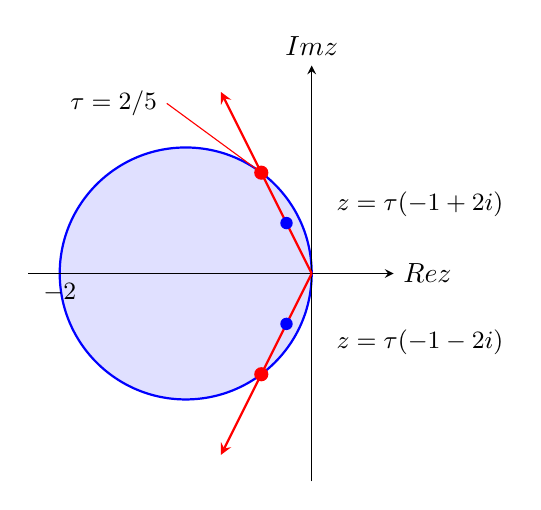
\begin{tikzpicture}[scale=1.6,>=stealth]
 \filldraw[fill=blue!12,draw=blue,thick] (-1,0) circle (1);
 \draw[->] (-2.25,0)--(.65,0) node[right] {\(\operatorname{Re}z\)};
 \draw[->] (0,-1.65)--(0,1.65) node[above] {\(\operatorname{Im}z\)};
 \draw[->,red,thick] (0,0)--(-.72,1.44);
 \draw[->,red,thick] (0,0)--(-.72,-1.44);
 \foreach \x/\y in {-.2/.4,-.2/-.4} \fill[blue] (\x,\y) circle (1.4pt);
 \foreach \x/\y in {-.4/.8,-.4/-.8} \fill[red] (\x,\y) circle (1.6pt);
 \draw[red] (-.4,.8)--(-1.15,1.35)
  node[left,black] {\small \(\tau=2/5\)};
 \node[right] at (.12,.55) {\small \(z=\tau(-1+2i)\)};
 \node[right] at (.12,-.55) {\small \(z=\tau(-1-2i)\)};
 \node[below] at (-2,0) {\small \(-2\)};
\end{tikzpicture}
\caption{The scaled eigenvalues travel along conjugate rays. The
points for \(\tau=1/5\) lie inside Euler's disk; the red points for
\(\tau=2/5\) lie on its boundary.}
\end{figure}

For stiff equations, these restrictions can require many steps even
when the solution of interest changes slowly. This motivates methods
with no step-size restriction for decay of the linear test equation.

\subsection{Backward Euler}

Backward Euler evaluates the slope at the new time and state:
\begin{equation}\label{eq:backward-euler-sep-18}
 x_{n+1}=x_n+\tau f(t_{n+1},x_{n+1}).
\end{equation}
For \(f(t,x)=Ax\),
\[
 (I-\tau A)x_{n+1}=x_n,
 \qquad G_{\mathrm{BE}}=(I-\tau A)^{-1}.
\]
Why is the inverse defined for every \(\tau>0\) if \(A\) is Hurwitz?
If \(I-\tau A\) were singular, there would be a nonzero \(v\) with
\(Av=\tau^{-1}v\). This would give a positive real eigenvalue of
\(A\), a contradiction.

The rational spectral mapping identity gives
\begin{equation}\label{eq:be-spectral-mapping-sep-18}
 \sigma(G_{\mathrm{BE}})
   =\left\{\frac{1}{1-\tau\lambda}:\lambda\in\sigma(A)\right\}.
\end{equation}
For completeness, if \(B=I-\tau A\) is invertible, its eigenvalues
are \(1-\tau\lambda\), and those of \(B^{-1}\) are their reciprocals.
This also follows by triangularizing \(A\); no diagonalizability
assumption is needed.

Thus the stability function and its non-strict domain are
\begin{equation}\label{eq:be-domain-sep-18}
 R_{\mathrm{BE}}(z)=\frac1{1-z},
 \qquad
 \mathcal D_{\mathrm{BE}}=\{z:|z-1|\geq1\}.
\end{equation}
The domain is the exterior, including the boundary, of the unit disk
centered at \(1\). The pole \(z=1\) is excluded automatically.
For \(\operatorname{Re}z<0\),
\[
 |1-z|^2=1-2\operatorname{Re}z+|z|^2>1,
\]
so \(|R_{\mathrm{BE}}(z)|<1\). Therefore, for every Hurwitz matrix
\(A\) and every fixed \(\tau>0\), backward Euler is asymptotically
stable. This is a statement about stability; resolving a solution
accurately can still require a small step.

\subsection{The implicit trapezoidal method}

The trapezoidal rule averages the old and new slopes:
\begin{equation}\label{eq:trapezoidal-sep-18}
 x_{n+1}=x_n+\frac{\tau}{2}
   \bigl(f(t_n,x_n)+f(t_{n+1},x_{n+1})\bigr).
\end{equation}
This is the \emph{implicit} trapezoidal method. Heun's method, the
explicit trapezoidal method from September 2, instead evaluates
the second slope at a forward Euler prediction.

For \(x'=Ax\), rearranging gives
\[
 \left(I-\frac\tau2 A\right)x_{n+1}
   =\left(I+\frac\tau2 A\right)x_n,
 \qquad
 G_{\mathrm{TR}}=
 \left(I-\frac\tau2 A\right)^{-1}\left(I+\frac\tau2 A\right).
\]
If \(A\) is Hurwitz, the inverse exists for every \(\tau>0\) by the
same argument as for backward Euler. Its eigenvalues are
\[
 \sigma(G_{\mathrm{TR}})
  =\left\{\frac{1+\tau\lambda/2}{1-\tau\lambda/2}:
       \lambda\in\sigma(A)\right\}.
\]
Hence
\begin{equation}\label{eq:trapezoidal-stability-function-sep-18}
 R_{\mathrm{TR}}(z)=\frac{1+z/2}{1-z/2}=\frac{2+z}{2-z}.
\end{equation}
Writing \(z=x+iy\),
\begin{align*}
 |R_{\mathrm{TR}}(z)|\leq1
 &\quad\Longleftrightarrow\quad |2+z|^2\leq|2-z|^2\\
 &\quad\Longleftrightarrow\quad (2+x)^2+y^2\leq(2-x)^2+y^2\\
 &\quad\Longleftrightarrow\quad x\leq0.
\end{align*}
Thus
\begin{equation}\label{eq:trapezoidal-domain-sep-18}
 \mathcal D_{\mathrm{TR}}=\{z:\operatorname{Re}z\leq0\},
 \qquad
 \mathcal S_{\mathrm{TR}}=\{z:\operatorname{Re}z<0\}.
\end{equation}
The pole \(z=2\) lies outside these sets. The trapezoidal method is
also asymptotically stable for every positive fixed step when \(A\)
is Hurwitz.

\begin{figure}[htbp]
\centering
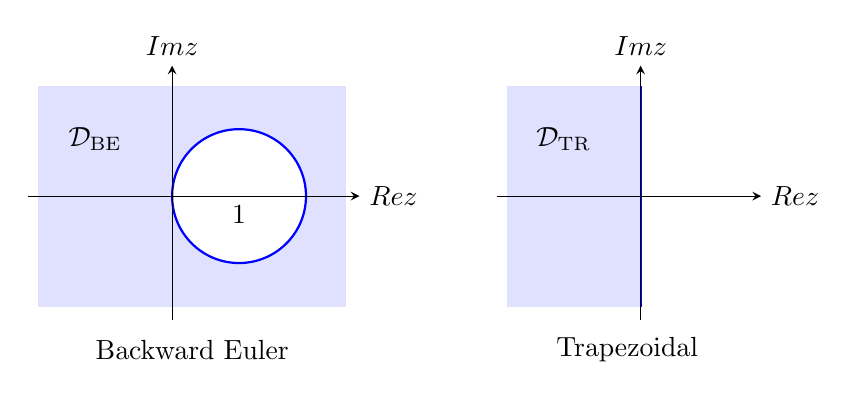
\begin{tikzpicture}[scale=.85,>=stealth]
 \begin{scope}
  \fill[blue!12] (-2,-1.65) rectangle (2.6,1.65);
  \filldraw[fill=white,draw=blue,thick] (1,0) circle (1);
  \draw[->] (-2.15,0)--(2.8,0) node[right] {\(\operatorname{Re}z\)};
  \draw[->] (0,-1.85)--(0,1.95) node[above] {\(\operatorname{Im}z\)};
  \node[below] at (1,0) {1};
  \node at (-1.15,.85) {\(\mathcal D_{\mathrm{BE}}\)};
  \node at (.3,-2.3) {Backward Euler};
 \end{scope}
 \begin{scope}[xshift=7cm]
  \fill[blue!12] (-2,-1.65) rectangle (0,1.65);
  \draw[blue,thick] (0,-1.65)--(0,1.65);
  \draw[->] (-2.15,0)--(1.8,0) node[right] {\(\operatorname{Re}z\)};
  \draw[->] (0,-1.85)--(0,1.95) node[above] {\(\operatorname{Im}z\)};
  \node at (-1.15,.85) {\(\mathcal D_{\mathrm{TR}}\)};
  \node at (-.2,-2.3) {Trapezoidal};
 \end{scope}
\end{tikzpicture}
\caption{The shaded stability domains extend to infinity. Both contain
the entire left half-plane; backward Euler also damps some modes in
the right half-plane, which is not faithful to the growth of those
exact modes.}
\end{figure}

\begin{definition}[\(A\)-stability]
 A method is \emph{\(A\)-stable} if its stability function is defined
 and satisfies \(|R(z)|\leq1\) throughout the open left half-plane.
\end{definition}

Backward Euler and the trapezoidal method are \(A\)-stable. Theorem~
\ref{thm:bounded-explicit-rk-sep-16} shows that no consistent explicit
RK method with finitely many stages can be \(A\)-stable.

\subsection{Oscillations: growth, damping, or constant amplitude}

Return to the skew-symmetric oscillator matrix
\(A=\left[\begin{smallmatrix}0&1\\-1&0\end{smallmatrix}\right]\)
from \eqref{eq:oscillator-sep-16}. The exact norm is constant. The
scalar amplification factors on the imaginary axis satisfy
\[
\begin{array}{c|c|c}
 \text{method}&|R(i\tau)|&\text{amplitude behavior}\\ \hline
 \text{forward Euler}&\sqrt{1+\tau^2}&\text{growth}\\
 \text{backward Euler}&(1+\tau^2)^{-1/2}&\text{decay}\\
 \text{trapezoidal}&1&\text{constant}
\end{array}
\]
For backward Euler,
\[
 \|x_n\|_2=(1+\tau^2)^{-n/2}\|x_0\|_2;
\]
the damping is artificial for this conservative problem.

For the trapezoidal method, put \(q=\tau/2\). Since \(A^2=-I\),
\[
 G_{\mathrm{TR}}
   =\frac{(1-q^2)I+2qA}{1+q^2},
 \qquad
 G_{\mathrm{TR}}^{\mathsf T}G_{\mathrm{TR}}=I.
\]
Thus the numerical update is an orthogonal rotation and preserves
\(\|x_n\|_2\) exactly. More generally, the same orthogonality follows
for every real skew-symmetric matrix \(A\), since the factors
\(I\pm qA\) commute.

\begin{figure}[htbp]
\centering
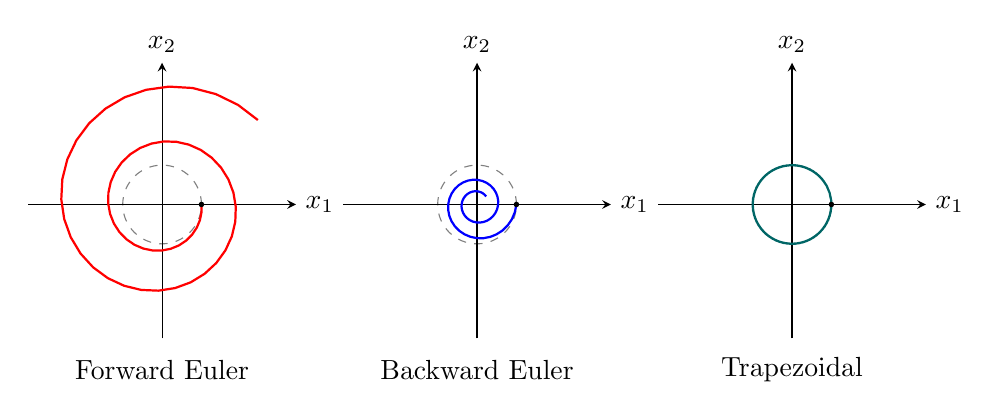
\begin{tikzpicture}[scale=.5,>=stealth]
\begin{scope}[xshift=0cm]
\draw[gray,dashed] (0,0) circle (1);
\draw[->] (-3.4,0)--(3.4,0) node[right] {\(x_1\)};
\draw[->] (0,-3.4)--(0,3.6) node[above] {\(x_2\)};
\node at (0,-4.2) {Forward Euler};
\draw[red,thick] plot coordinates {
(1.00000,0.00000) (1.00000,-0.20000) (0.96000,-0.40000) (0.88000,-0.59200) (0.76160,-0.76800) (0.60800,-0.92032)
(0.42394,-1.04192) (0.21555,-1.12671) (-0.00979,-1.16982) (-0.24375,-1.16786) (-0.47732,-1.11911) (-0.70115,-1.02364)
(-0.90588,-0.88341) (-1.08256,-0.70224) (-1.22301,-0.48573) (-1.32015,-0.24113) (-1.36838,0.02290) (-1.36380,0.29658)
(-1.30448,0.56934) (-1.19061,0.83023) (-1.02457,1.06836) (-0.81089,1.27327) (-0.55624,1.43545) (-0.26915,1.54670)
(0.04019,1.60053) (0.36029,1.59249) (0.67879,1.52043) (0.98288,1.38467) (1.25981,1.18810) (1.49743,0.93613)
(1.68466,0.63665) (1.81199,0.29972) (1.87193,-0.06268) (1.85940,-0.43707) (1.77198,-0.80895) (1.61019,-1.16334)
(1.37752,-1.48538) (1.08045,-1.76089) (0.72827,-1.97698) (0.33287,-2.12263) (-0.09165,-2.18921) (-0.52949,-2.17088)
(-0.96367,-2.06498) (-1.37666,-1.87224) (-1.75111,-1.59691) (-2.07049,-1.24669) (-2.31983,-0.83259) (-2.48635,-0.36862)
(-2.56007,0.12865) (-2.53434,0.64066) (-2.40621,1.14753) (-2.17671,1.62877) (-1.85095,2.06411) (-1.43813,2.43430)
(-0.95127,2.72193) (-0.40688,2.91218) (0.17555,2.99356) (0.77427,2.95845) (1.36596,2.80360) (1.92668,2.53040)
(2.43276,2.14507)
};
\fill (1,0) circle (2pt);
\end{scope}
\begin{scope}[xshift=8cm]
\draw[gray,dashed] (0,0) circle (1);
\draw[->] (-3.4,0)--(3.4,0) node[right] {\(x_1\)};
\draw[->] (0,-3.4)--(0,3.6) node[above] {\(x_2\)};
\node at (0,-4.2) {Backward Euler};
\draw[blue,thick] plot coordinates {
(1.00000,0.00000) (0.96154,-0.19231) (0.88757,-0.36982) (0.78232,-0.52629) (0.65102,-0.65649) (0.49973,-0.75644)
(0.33504,-0.82344) (0.16380,-0.85620) (-0.00715,-0.85477) (-0.17126,-0.82052) (-0.32246,-0.75603) (-0.45545,-0.66494)
(-0.56581,-0.55178) (-0.65016,-0.42175) (-0.70626,-0.28050) (-0.73303,-0.13389) (-0.73059,0.01223) (-0.70014,0.15226)
(-0.64393,0.28104) (-0.56512,0.39406) (-0.46760,0.48758) (-0.35585,0.55875) (-0.23471,0.60570) (-0.10920,0.62754)
(0.01568,0.62440) (0.13515,0.59737) (0.24483,0.54840) (0.34088,0.48023) (0.42012,0.39620) (0.48015,0.30017)
(0.51941,0.19629) (0.53718,0.08885) (0.53361,-0.01787) (0.50965,-0.11980) (0.46701,-0.21320) (0.40805,-0.29481)
(0.33566,-0.36194) (0.25315,-0.41257) (0.16407,-0.44538) (0.07211,-0.45981) (-0.01909,-0.45599) (-0.10605,-0.43478)
(-0.18558,-0.39766) (-0.25491,-0.34668) (-0.31178,-0.28432) (-0.35447,-0.21343) (-0.38188,-0.13706) (-0.39355,-0.05835)
(-0.38963,0.01958) (-0.37088,0.09376) (-0.33858,0.16147) (-0.29451,0.22037) (-0.24080,0.26853) (-0.17990,0.30451)
(-0.11442,0.32740) (-0.04706,0.33681) (0.01952,0.33291) (0.08279,0.31635) (0.14044,0.28826) (0.19048,0.25016)
(0.23126,0.20391)
};
\fill (1,0) circle (2pt);
\end{scope}
\begin{scope}[xshift=16cm]
\draw[gray,dashed] (0,0) circle (1);
\draw[->] (-3.4,0)--(3.4,0) node[right] {\(x_1\)};
\draw[->] (0,-3.4)--(0,3.6) node[above] {\(x_2\)};
\node at (0,-4.2) {Trapezoidal};
\draw[teal!80!black,thick] plot coordinates {
(1.00000,0.00000) (0.98020,-0.19802) (0.92158,-0.38820) (0.82646,-0.56300) (0.69861,-0.71551) (0.54309,-0.83968)
(0.36606,-0.93059) (0.17454,-0.98465) (-0.02390,-0.99971) (-0.22139,-0.97519) (-0.41011,-0.91204) (-0.58259,-0.81276)
(-0.73200,-0.68131) (-0.85242,-0.52286) (-0.93907,-0.34372) (-0.98854,-0.15095) (-0.99886,0.04779) (-0.96962,0.24463)
(-0.90197,0.43179) (-0.79861,0.60185) (-0.66362,0.74807) (-0.50234,0.86467) (-0.32117,0.94702) (-0.12728,0.99187)
(0.07164,0.99743) (0.26774,0.96349) (0.45323,0.89140) (0.62077,0.78400) (0.76372,0.64555) (0.87643,0.48153)
(0.95443,0.29845) (0.99462,0.10354) (0.99543,-0.09546) (0.95682,-0.29069) (0.88031,-0.47440) (0.76894,-0.63933)
(0.62711,-0.77893) (0.46045,-0.88769) (0.27555,-0.96129) (0.07974,-0.99682) (-0.11923,-0.99287) (-0.31347,-0.94960)
(-0.49530,-0.86872) (-0.65752,-0.75344) (-0.79370,-0.60832) (-0.89844,-0.43910) (-0.96760,-0.25250) (-0.99844,-0.05590)
(-0.98973,0.14292) (-0.94183,0.33608) (-0.85663,0.51593) (-0.73751,0.67534) (-0.58917,0.80801) (-0.41750,0.90867)
(-0.22930,0.97336) (-0.03202,0.99949) (0.16654,0.98604) (0.35849,0.93353) (0.53625,0.84406) (0.69277,0.72116)
(0.82186,0.56969)
};
\fill (1,0) circle (2pt);
\end{scope}
\end{tikzpicture}
\caption{The same oscillator and initial value \((1,0)\), with \(\tau=.2\) for 60 steps in each panel, on identical scales. The dashed circle is the exact orbit. Trapezoidal vertices remain on the circle; the straight segments only join successive iterates.}
\end{figure}

Amplitude preservation does not imply exact phase. On the scalar
mode \(y'=iy\),
\[
 R_{\mathrm{TR}}(i\tau)
   =\exp\left(2i\arctan\frac\tau2\right),
 \qquad
 2\arctan\frac\tau2=\tau-\frac{\tau^3}{12}+O(\tau^5).
\]
The exact phase advance is \(\tau\). The numerical frequency is
\[
 \frac{2}{\tau}\arctan\frac{\tau}{2}.
\]
For the real oscillator drawn here, the
rotation is clockwise, with this same angle magnitude.
Purely imaginary eigenvalues alone do not imply conservation of the
Euclidean norm for an arbitrary matrix; skew-symmetry is the property
used in this example.

\subsection{Damping very stiff modes: an additional comparison}

Both implicit methods allow arbitrary steps for linear stability,
but they behave differently when \(z=-r\) with \(r\gg1\):
\[
 R_{\mathrm{BE}}(-r)=\frac1{1+r}\longrightarrow0,
 \qquad
 R_{\mathrm{TR}}(-r)=\frac{1-r/2}{1+r/2}\longrightarrow-1.
\]
The exact factor \(e^{-r}\) is very small. Backward Euler strongly
damps such a mode, while the trapezoidal method can produce slowly
decaying sign alternations when the step is large compared with the
mode's decay time.

\begin{figure}[htbp]
\centering
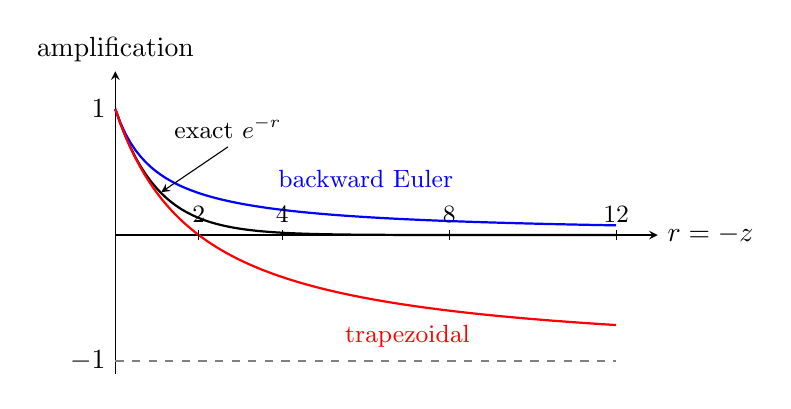
\begin{tikzpicture}[xscale=.53,yscale=1.6,>=stealth]
 \draw[->] (0,0)--(13,0) node[right] {\(r=-z\)};
 \draw[->] (0,-1.1)--(0,1.3) node[above] {amplification};
 \draw[dashed,gray] (0,-1)--(12,-1);
 \draw[black,thick,domain=0:12,samples=100] plot (\x,{exp(-\x)});
 \draw[blue,thick,domain=0:12,samples=100] plot (\x,{1/(1+\x)});
 \draw[red,thick,domain=0:12,samples=100] plot (\x,{(1-\x/2)/(1+\x/2)});
 \foreach \x in {2,4,8,12} \draw (\x,.04)--(\x,-.04) node[above=3pt] {\small \x};
 \node[left] at (0,1) {1}; \node[left] at (0,-1) {\(-1\)};
 \node[blue] at (6,.45) {\small backward Euler};
 \node[red] at (7,-.8) {\small trapezoidal};
 \node at (2.7,.85) {\small exact \(e^{-r}\)};
 \draw[->] (2.7,.7)--(1.1,.34);
\end{tikzpicture}
\caption{Signed amplification factors along the negative real axis.
The trapezoidal factor changes sign at \(r=2\) and approaches \(-1\);
backward Euler's factor approaches zero.}
\end{figure}

An \(A\)-stable method is called \emph{\(L\)-stable} if in addition
\(R(z)\to0\) as \(|z|\to\infty\) in the left half-plane. Thus backward
Euler is \(L\)-stable and the trapezoidal method is not. This additional
notion explains their different behavior on very fast decaying modes.

\subsection{Implicit Runge--Kutta methods and their tableaux}

The stage and update formulas are the same as in
\eqref{eq:rk-stages-sep-02}--\eqref{eq:rk-update-sep-02}:
\begin{align*}
 k_i&=f\left(t_n+c_i\tau,
      x_n+\tau\sum_{j=1}^{s}a_{ij}k_j\right),
      \qquad i=1,\ldots,s,\\
 x_{n+1}&=x_n+\tau\sum_{i=1}^{s}b_i k_i.
\end{align*}
For an implicit method, the stage equations need not be solvable by
successive explicit evaluations: a stage may depend on itself or on
other unknown stages. They generally require solving algebraic
systems, nonlinear if \(f\) is nonlinear. The internal consistency
relation remains \(c=\mathsf A\mathbf1\).

\subsubsection{Backward Euler as a one-stage RK method}

Take \(a_{11}=b_1=c_1=1\):
\[
 \begin{array}{c|c}1&1\\\hline &1\end{array}.
\]
Then
\[
 k_1=f(t_n+\tau,x_n+\tau k_1),\qquad x_{n+1}=x_n+\tau k_1,
\]
which is exactly \eqref{eq:backward-euler-sep-18}. The coefficient
\(a_{11}=1\) makes the sole stage implicit.

\subsubsection{Trapezoidal rule as a two-stage RK method}

Its tableau is
\[
 \begin{array}{c|cc}
  0&0&0\\
  1&\tfrac12&\tfrac12\\\hline
   &\tfrac12&\tfrac12
 \end{array},
 \qquad
 \mathsf A=\begin{bmatrix}0&0\\\tfrac12&\tfrac12\end{bmatrix}.
\]
Indeed,
\begin{align*}
 k_1&=f(t_n,x_n),\\
 k_2&=f\left(t_n+\tau,x_n+\frac\tau2k_1+\frac\tau2k_2\right),\\
 x_{n+1}&=x_n+\frac\tau2(k_1+k_2).
\end{align*}
The argument of \(f\) in the second stage is \(x_{n+1}\), so this
recovers \eqref{eq:trapezoidal-sep-18}. Its weights satisfy
\(b^{\mathsf T}\mathbf1=1\) and \(b^{\mathsf T}c=1/2\), giving order
two by the earlier order conditions. In contrast, backward Euler has
\(b^{\mathsf T}c=1\), so it has only order one.

\subsection{Derivation of the general RK stability function}

On \(y'=\lambda y\), each stage satisfies
\[
 k_i=\lambda y_n+z\sum_{j=1}^s a_{ij}k_j,
 \qquad z=\tau\lambda.
\]
Collecting the slopes into \(k=(k_1,\ldots,k_s)^{\mathsf T}\) gives
\[
 (I-z\mathsf A)k=\lambda y_n\mathbf1.
\]
Whenever \(I-z\mathsf A\) is invertible, substitution into the update
produces
\begin{align*}
 y_{n+1}
  &=y_n+\tau b^{\mathsf T}k\\
  &=\left(1+z b^{\mathsf T}(I-z\mathsf A)^{-1}\mathbf1\right)y_n.
\end{align*}
Thus the formula from September 4 applies to both explicit and
implicit RK schemes:
\begin{equation}\label{eq:general-rk-stability-sep-18}
 \boxed{R(z)=1+z b^{\mathsf T}(I-z\mathsf A)^{-1}\mathbf1.}
\end{equation}
For implicit methods the inverse is generally a rational matrix
function, so \(R\) need not be a polynomial. The determinant lemma
also gives
\[
 R(z)=\frac{\det(I-z\mathsf A+z\mathbf1b^{\mathsf T})}
             {\det(I-z\mathsf A)}.
\]
The numerator and denominator have degree at most \(s\), before
possible cancellations. At a singular stage matrix, the original
stage equations must still be checked; a removable singularity in a
simplified scalar formula does not by itself make the stages uniquely
solvable.

For backward Euler this yields
\(R(z)=1+z/(1-z)=1/(1-z)\). For the trapezoidal tableau, solve
\[
 (I-z\mathsf A)w=\mathbf1
 \quad\Longrightarrow\quad
 w_1=1,\qquad w_2=\frac{1+z/2}{1-z/2}.
\]
Then \(R(z)=1+z(w_1+w_2)/2=(1+z/2)/(1-z/2)\), as above.
Implicitness permits \(A\)-stability but does not guarantee it; the
actual rational stability function must be examined.

\subsection{Connection with collocation}

The lecture lists collocation as the next topic. The following short
construction explains its connection with the implicit RK formulas.
Choose distinct nodes \(c_1,\ldots,c_s\in[0,1]\) and let \(u\) be a
polynomial of degree at most \(s\) on one time step such that
\[
 u(t_n)=x_n,\qquad
 u'(t_n+c_i\tau)=f(t_n+c_i\tau,u(t_n+c_i\tau)).
\]
Let \(\ell_j(\theta)\) be the Lagrange basis at these nodes and set
\(k_j=u'(t_n+c_j\tau)\). Interpolation of \(u'\), followed by
integration, gives
\[
 u(t_n+\theta\tau)
  =x_n+\tau\sum_{j=1}^s
       \left(\int_0^\theta\ell_j(\xi)\,d\xi\right)k_j.
\]
Evaluating at the nodes and at \(\theta=1\) produces the RK coefficients
\begin{equation}\label{eq:collocation-coefficients-sep-18}
 a_{ij}=\int_0^{c_i}\ell_j(\xi)\,d\xi,
 \qquad b_j=\int_0^1\ell_j(\xi)\,d\xi.
\end{equation}
The single node \(c_1=1\) gives backward Euler. The two nodes \(0,1\)
give \(\ell_1(\theta)=1-\theta\) and \(\ell_2(\theta)=\theta\), hence
exactly the trapezoidal tableau above.

\begin{figure}[htbp]
\centering
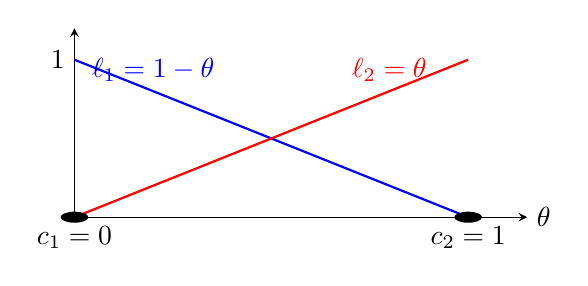
\begin{tikzpicture}[xscale=5,yscale=2,>=stealth]
 \draw[->] (0,0)--(1.15,0) node[right] {\(\theta\)};
 \draw[->] (0,0)--(0,1.2);
 \draw[blue,thick] (0,1)--(1,0);
 \draw[red,thick] (0,0)--(1,1);
 \node[blue,above] at (.2,.8) {\(\ell_1=1-\theta\)};
 \node[red,above] at (.8,.8) {\(\ell_2=\theta\)};
 \fill (0,0) circle (1pt) node[below] {\(c_1=0\)};
 \fill (1,0) circle (1pt) node[below] {\(c_2=1\)};
 \node[left] at (0,1) {1};
\end{tikzpicture}
\caption{The endpoint Lagrange basis for trapezoidal collocation.
Each basis function has integral \(1/2\), giving the two equal weights;
its integral up to each node gives the corresponding tableau row.}
\end{figure}
